%中間審査概要テンプレート ver. 3.0

\documentclass[uplatex,twocolumn,dvipdfmx]{jsarticle}
\usepackage[top=22mm,bottom=22mm,left=22mm,right=22mm]{geometry}
\setlength{\columnsep}{10mm}
\usepackage[T1]{fontenc}
\usepackage{txfonts}
\usepackage[expert,deluxe]{otf}
\usepackage[dvipdfmx,hiresbb]{graphicx}
\usepackage[dvipdfmx]{hyperref}
\usepackage{pxjahyper}
\usepackage{secdot}





%タイトルと学生番号,名前だけ編集すること
\title{\vspace{-5mm}\fontsize{14pt}{0pt}\selectfont 学生生活実態調査のためのデータマイニング手法の提案}
\author{\normalsize プロジェクトマネジメントコース 矢吹研究室 1342045 川手元稀}
\date{}
\pagestyle{empty}
\begin{document}
\fontsize{10.5pt}{\baselineskip}\selectfont
\maketitle





%以下が本文
\section{背景}
千葉工業大学では2001年から学生の意識や考え方を調査するために,毎年「学生生活アンケート」を行っている.
このアンケートの結果は,調査報告書としてまとめ,津田沼校舎や新習志野校舎の図書館等に掲示している.
しかし,調査報告書を見た際,学生の意識や考え方に関する分析や解析が行われていないと感じた.
このアンケートの本来の目的は学生の意識や考え方を調査するためのアンケートである\cite{a}.
そこで,学生の意識や考え方を掴むためには,収集したデータの分析や解析が必要であると考えた.
そのためには,データマイニングの手法を利用することが良いと考えた.学生はどのような意識で学校に来ているのか.
また,学生はどのような考え方で学校に来ているのか.「学生生活アンケート」の結果を更に発展させたいと思い,このテーマに定めた.


\begin{figure}[htbp]
  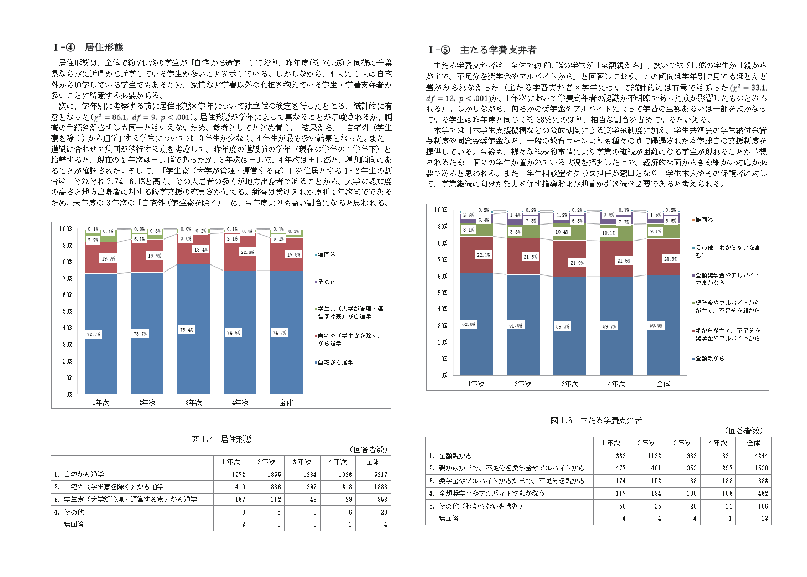
\includegraphics[width=7.5cm]{questionnairesurvey.pdf}
\caption{調査報告書の例}\label{調査報告書}
\end{figure}

\section{目的}
千葉工業大学の学生に2015年度版「学生生活アンケート」を100人分実施する.集めたデータをデータマイニングの手法を用いて学生の意識や考え方を明らかにする.
明らかにした結果を人々に伝わりやすく可視化することを目的とする.

\section{手法}
本研究は4段階に分かれる.

\begin{enumerate}
\item 千葉工業大学が実施した2015年度版「学生生活アンケート」をGoogleフォームにて作成する.
\item 千葉工業大学の学生100人分のアンケートを集める.
\item 学生の意識や考え方に関するデータに注目し,独自に分析,解析する.
\item 新たな解析法の提案をする.
\end{enumerate}

\section{想定される成果物}
以下の提案事項が考えられる.
\begin{enumerate}
\item 学生の考え方や意識を可視化できるような手法の提案
\item 報告書を見た人が今の学生がどのようなことを望んでいるのか一目でわかるようなまとめ方の提案
\item 千葉工業大学の更なる発展
\end{enumerate}

\section{進捗状況}
手法の1段階目を終了し,研究室内で22人分のアンケートを実施した.現在解析中である.
\section{今後の計画}

今後の計画は以下の通りである.
\begin{table}[hbtp]
  \caption{今後の計画}
  \label{table:data_type}
  \centering
  \begin{tabular}{cc}
    \hline
    日程 & 内容  \\ \hline \hline
    10月 & 残り78人分のアンケートを実施 \\
    11月 & 回収したデータの分析,解析 \\
    12月 & 学生の意識と考え方が最も可視化出来た結果を提案する \\
    1月 & 論文の執筆,発表資料の作成 \\
2月 & 論文発表\\
 \hline
  \end{tabular}
\end{table}


\bibliographystyle{junsrt}
\bibliography{biblio}%「biblio.bib」というファイルが必要.

\end{document}
